
\subsection{N-band imaging}
\label{sec:recipes_img_n}

\subsubsection{N-band imaging flatfield}
\label{sssec:n_img_flatfield}

The purpose of the flat-field calibration is to determine
pixel-to-pixel gain variations and large scale illumination variations
(due to inhomogeneities of optical elements in the telescope or
instrument). Calibration frames are obtained either during day time
using the black-body lamp of the \ac{WCU} (internal flats) or by taken
images of the twilight sky (twilight flats). Advantages and
disadvantages of the two types of flat are discussed in
\cite{METIS-calibration_plan}.

MIR detectors are typically unstable in that they show gain
fluctuations on rather short time scales, hence science exposures may
have a different flat-field structure from those captured by the
calibration flats.  While the GeoSnap detector is expected to be more
stable than the AQUARIUS detector, its stability properties need to be
studied further in order to assess whether science images can be flat
fielded.  N-band flat fields will be taken in any case for quality
control and monitoring purposes.

Since the operational concept for twilight flats needs to be refined
during commissioning at the telescope, the current recipe design is
primarily valid for internal flats.

This recipe creates a master flat for the GeoSnap detector (N-band
imaging) from lamp or sky images matched by various setup parameters
as detailed below.  A set of internal flats includes a number of
exposures with \CODE{LAMP OFF}, which will be used for dark
subtraction. For twilight flats a master dark will be subtracted. The
master flat is obtained by the slope of a linear fit of the pixel
values against the illumination level of the exposures.

The quality control parameters give various statistics for each input
frame (mean, standard deviation, etc.), the standard deviation of the
normalised master flat and the number of bad pixels identified by the
recipe. If a bad-pixel map is provided on input, it is updated,
otherwise a new one is created.

\begin{recipedef}
  Name:                & \REC{metis_n_img_flat}                                     \\
  Purpose:             & Create master flat field for the N-band imaging detector.  \\
  Requirements:        & \REQ{METIS-6098}                                           \\
  Type:                & Calibration                                                \\
  Templates:           & \TPL{METIS_img_n_cal_LampFlat}                             \\
                       & \TPL{METIS_all_cal_TwilightFlat}                           \\
  Input data:          & Flat field images taken with lamp or sky.                  \\
                       & Master dark (for twilight flats)                           \\
                       & Bad pixel map                                              \\
  Matched keywords:    & Detector ID                                                \\
                       & Filter ID                                                  \\
                       & ADC ID                                                     \\
                       & possibly others (e.g.\ coronagraphic mask, \TBD)           \\
  Recipe parameters:   & Combination method (\texttt{mean}, \texttt{median},
                         \texttt{sigclip}, \dots)                                \\
                       & Parameters for combination methods                         \\
                       & Threshold for bad-pixel identification                     \\
  Algorithm:           & For internal flats: combine \CODE{LAMP OFF} exposures to dark. \\
                       & Subtract internal dark or master dark from flat exposures. \\
                       & Fit slope of pixel values against illumination level.      \\
                       & Add pixels with significant deviations to bad pixel map.   \\
  Output data:         & \PROD{MASTER_IMG_FLAT_GEO}                                 \\
                       & \PROD{BADPIX_MAP_GEO}                                      \\
  Expected accuracies: & \TBD                                                       \\
  QC1 parameters:      & \QC{QC N MASTERFLAT RMS}                                   \\
                       & \QC{QC N FLAT NBADPIX}                                     \\
                       & \QC{QC N FLAT MEAN ##}                                     \\
                       & \QC{QC N FLAT RMS ##}                                      \\
  hdrl function        & \CODE{hdrl_bpm_fit_compute}                                \\
                       & \CODE{hdrl_imagelist_collapse}                             \\
                       & \CODE{hdrl_imagelist_sub_image}                            \\
\end{recipedef}

\begin{figure}[hb]
  \centering
  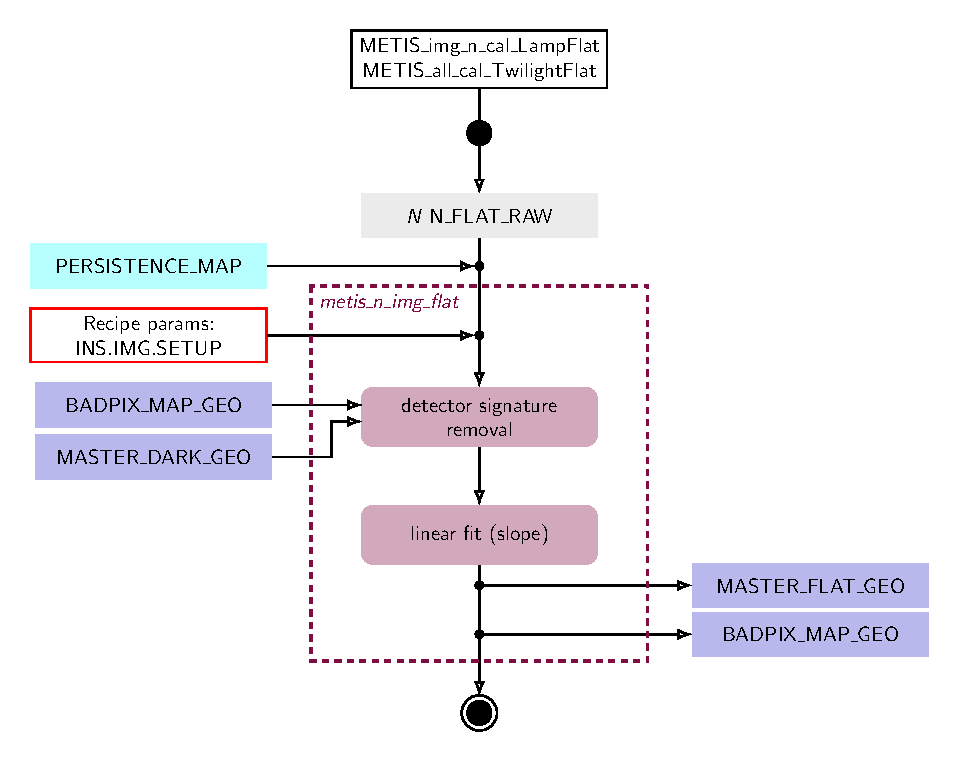
\includegraphics[width=0.6\textwidth]{metis_n_img_flat}
  \caption[Recipe: \REC{metis_n_img_flat}]{\REC{metis_n_img_flat} --
    creation of \CODE{IMG_N} master flatfield\\
    \TODO{Update (`nq' to `n')}}
  \label{fig:metis_n_img_flat}
\end{figure}


%%% Local Variables:
%%% TeX-master: "METIS_DRLD"
%%% End:
